\capitulo{4}{Conceptos teóricos}

\section{Machine Learning y Deep Learning}
El proyecto se ha basado en el uso del \emph{machine learning}, y más en concreto, en una de sus ramas: el \emph{deep learning}.

\subsection{Machine Learning}
El aprendizaje automático, también conocido como \emph{machine learning} en inglés, \cite{bobadilla2021machine} se centra en conseguir que con unos datos iniciales, y aplicado algún tipo de algoritmo o técnica, un computador sea capaz de aprender.

Para conseguir esto, adopta el proceso de observación y aprendizaje utilizado por los seres vivos, de forma que cuantos más ``sucesos'' haya, mayor conocimiento podrá obtener, es decir, cuanto mayor sea el número de datos con el que se cuente, los resultados obtenidos también serán mejores. En la Figura \ref{f:esquemaML} se puede ver detalladamente como funciona el \emph{machine learning}.

\begin{figure}[h]
    \centering
    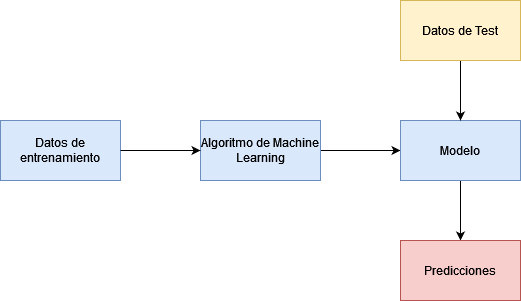
\includegraphics[scale=0.7]{img/Esquema_ML.png}
    \caption{Esquema Algoritmos Machine Learning (Realización Propia).}
    \label{f:esquemaML}
\end{figure}

Este tipo de aprendizaje debe utilizarse en problemas donde se tengan multitud de datos y multitud de escenarios y posibilidades, y que a su vez se puedan modelar todas sus soluciones de forma matemática.

Finalmente, los tipos de \emph{machine learning}, según el problema al que se enfrente, son:
\begin{itemize}
    \item \textbf{Aprendizaje supervisado:} cada dato del conjunto de datos va acompañado de la clase a la que pertenece.
    \item \textbf{Aprendizaje no supervisado:} se desconoce la clase a la que pertenece cada dato.
    \item \textbf{Aprendizaje semisupervisado:} en el conjunto de datos, se conocerá la clase de alguno de los datos, mientras que de otros no.
    \item \textbf{Aprendizaje por refuerzo:} el algoritmo aprende en base a sus aciertos y fallos, mediante un sistema de recompensas y penalizaciones.
\end{itemize}

\subsection{Deep Learning}
El aprendizaje profundo, también conocido como \emph{deep learning} en inglés, \cite{bobadilla2021machine} es una de las ramas del \emph{machine learning} que se basa en el sistema nervioso humano, donde las neuronas están conectadas entre sí y cada una de ellas se encarga de una tarea en específico.

Esta estructura permite que ciertas zonas se encarguen de detectar ciertos patrones o características de los datos, lo que permite una gran mejoría con respecto al \emph{machine learning}, ya que esta estructura otorga a la red la posibilidad de aprender de manera automática, además de conseguir mejoras de rendimiento.

\section{Redes Neuronales Artificiales}
Las redes neuronales artificiales \cite{izaurieta2000redes} buscan recrear el sistema nervioso del ser humano, donde existen multitud de neuronas conectadas entre sí, y que intercambian pulsos.

En una red neuronal artificial existen multitud de neuronas artificiales conectadas entre sí por un enlace, que habitualmente suele llevar un peso asociado, consiguiendo así que otra neurona se active según el pulso que le llegue por sus enlaces.

Durante el proceso de entrenamiento, y de manera iterativa, se van modificando estos pesos, buscando los valores óptimos que minimicen alguna función de error o pérdida. Es la forma en la que red ``aprende'' a partir de los datos que se le prestan.

Según como fluyan los datos en la red, se distinguen principalmente dos tipos:
\begin{itemize}
    \item \textbf{Red neuronal prealimentada:} los datos siempre van hacia delante pasando por diferentes capas hasta llegar a la capa de salida. Durante todo este proceso no se permiten ni bucles ni volver hacia atrás, es decir, la información siempre se mueve hacia la siguiente capa. La Figura \ref{f:redneuronal} muestra de una manera más gráfica cómo se mueve la información. Este tipo de red es el más básico y se usa principalmente en problemas de clasificación y regresión.
    \item \textbf{Red neuronal recurrente:} permite que a lo largo de la red haya bucles o que se pueda avanzar hacia una capa anterior, otorgando a las neuronas una memoria interna que permitirá ir adaptándose según lleguen nuevos datos. Es por ello que se utiliza principalmente en problemas con datos secuenciales o \emph{data stream}.
    
\end{itemize}
\begin{figure}[h]
 \centering
  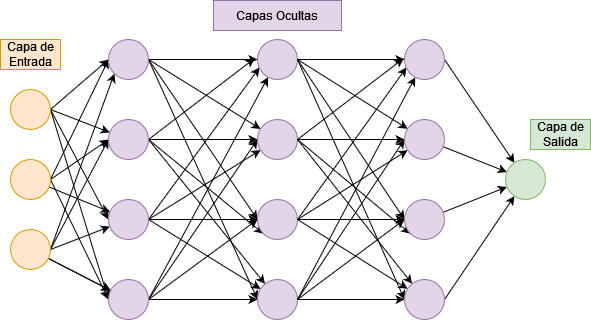
\includegraphics[width=0.8\textwidth]{img/RedNeuronal.png}
 \caption{Ejemplo Red Neuronal Artificial (Realización Propia)}
 \label{f:redneuronal}
\end{figure}

\subsection{Redes Neuronales Convolucionales}
Las redes neuronales convolucionales \cite{prieto2019redes}, también conocidas como CNN (por sus siglas en inglés \emph{Convolutional Neural Network}), son la variante de las redes neuronales artificiales más extendidas y utilizadas en la actualidad. Esto se debe al gran rendimiento que se obtiene en aquellos casos donde los datos se encuentren en cuadrícula, como un \emph{array} o matriz. Sus principales usos son en la clasificación de imágenes o en la detección de objetos. Es por ello, que, pesé a que existan muchas más variantes de redes neuronales, se ha empleado este tipo durante el desarrollo del proyecto. 

Este tipo de red se basa en aplicar dos operaciones diferentes: convolución y \emph{pooling}.

\subsubsection{Convolución}
La convolución \cite{prieto2019redes} es una operación que busca obtener características de los datos para que puedan ser aprendidos por la red neuronal. Para ello se utiliza una matriz, comúnmente denominada \emph{kernel}, que recorre todas las celdas de los valores de entrada y calcula, junto con las celdas de su alrededor, el producto escalar y dicho valor se almacena en el \emph{kernel}. De esta forma se va completando, y obteniendo una matriz, generalmente, de un tamaño menor que el de los datos de entrada.

En la Figura \ref{f:convo} se puede ver como funciona esta operación usando un \emph{kernel} de tamaño 3x3 sobre los datos iniciales.

\begin{figure}[h]
 \centering
  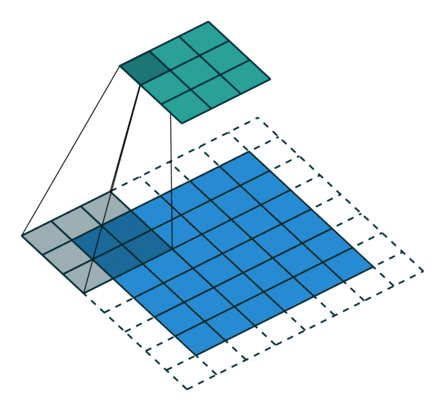
\includegraphics[width=0.6\textwidth]{img/Convo.png}
 \caption{Operación de Convolución \cite{wiki:convo}}
 \label{f:convo}
\end{figure}

\subsubsection{Pooling}
La operación \emph{pooling} \cite{prieto2019redes} busca reducir la dimensionalidad de la matriz de características obtenida en la operación anterior, de forma que queden aquellas más relevantes y se disminuya la carga computacional de la red neuronal.

Para ello, se divide el \emph{kernel} en una malla de un tamaño en específico, en la que, para cada celda, se devuelve un valor, que habitualmente suele ser el valor máximo o el valor medio; ya que según el problema a resolver puede ser mejor solución el uso del valor máximo, puesto que resalta las características más importantes, o el valor medio, que devuelve el promedio de las características.

En la Figura \ref{f:pooling} se puede observar un ejemplo de \emph{pooling} aplicando una malla de 2x2 y devolviendo por cada celda el valor máximo.

\begin{figure}[h]
 \centering
  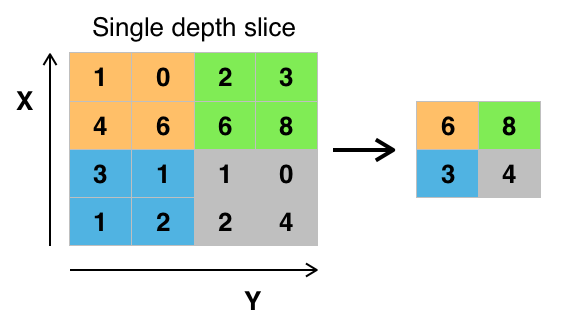
\includegraphics[width=0.7\textwidth]{img/pooling.png}
 \caption{Operación de \emph{Pooling} \cite{wiki:pooling}}
 \label{f:pooling}
\end{figure}

\section{Conjunto de Datos Desbalanceado}
En problemas de clasificación, cuando se quiere construir un modelo aplicando \emph{deep learning} es importante contar con una gran cantidad de datos de cada una de las clases. Aunque esto es, en algunos casos, difícil, por ejemplo, en medicina es más común que la gente este sana a que la gente esté enferma, por lo que en este conjunto de datos sería difícil de tener un número de personas equilibrado de ambas clases o el número de muestras equitativo de ambas clases sería limitado. A esto se le conoce como conjunto de datos desbalanceado o desequilibrado.

Ante estos inconvenientes, suele ser recomendable y eficiente aplicar alguna de las tres estrategias siguientes \cite{Na8_2020}:
\begin{itemize}
    \item \textbf{Submuestreo:} consiste en reducir el número de datos de la clase mayoritaria para tener ambas clases con el mismo número de registros.
    \item \textbf{Sobremuestreo:} se basa en generar nuevos datos de la clase minoritaria para poder equilibrar los datos de cada clase. Estos datos pueden ser repitiendo los mismos datos o creando nuevos ``sintéticos'', ya que según el problema puede ser mejor utilizar una técnica u otra.
    \item \textbf{Sobremuestreo y submuestreo}: se aplica en primer lugar el sobremuestreo para equilibrar ambas clases, y a continuación, aplicar el submuestreo sobre todos los datos para eliminar aquellos que estén repetidos o sean muy similares.
\end{itemize}

